%DO NOT MESS AROUND WITH THE CODE ON THIS PAGE UNLESS YOU %REALLY KNOW WHAT YOU ARE DOING
\chapter*{Experimental Research}
\addcontentsline{toc}{chapter}{Experimental Research}


\section{ Dependence of wind speed and frequency on Ambient noise } \label{ Dependence of wind speed and frequency on Ambient noise } 
\noindent  The ambient noise level versus frequency for wind speeds of 5, 10, 15, 20, 25 and 30 kn is plotted. In-order to obtain the figure (1), we assumed the biological, rainfall and self noise level to be -99 dB and the frequency in the range of 1 Hz to 1 MHz was considered.

\noindent Noise Level generally decreases with  increasing frequency, from figure (1) we see that between 1 Hz to 100 kHz, noise level reduces from 120 dB to 25 dB. Noise Level decreases at great depths since most noise sources are at the surface. Ambient noise is greater in shallow water (noise is trapped between sea floor and the ocean surface). From the observation, we can say that as the wind speed increases, noise level increases in the frequency range 300 Hz to 100 kHz. This is due to the bubbles created by wind generated surface agitation.  At lower frequencies, it is the oscillation of bubble clouds themselves that are considered to be the source of sound, while at higher frequencies the excitation of resonant oscillations by individual bubbles is the source of sound.

\begin{figure}[H]
\centering
{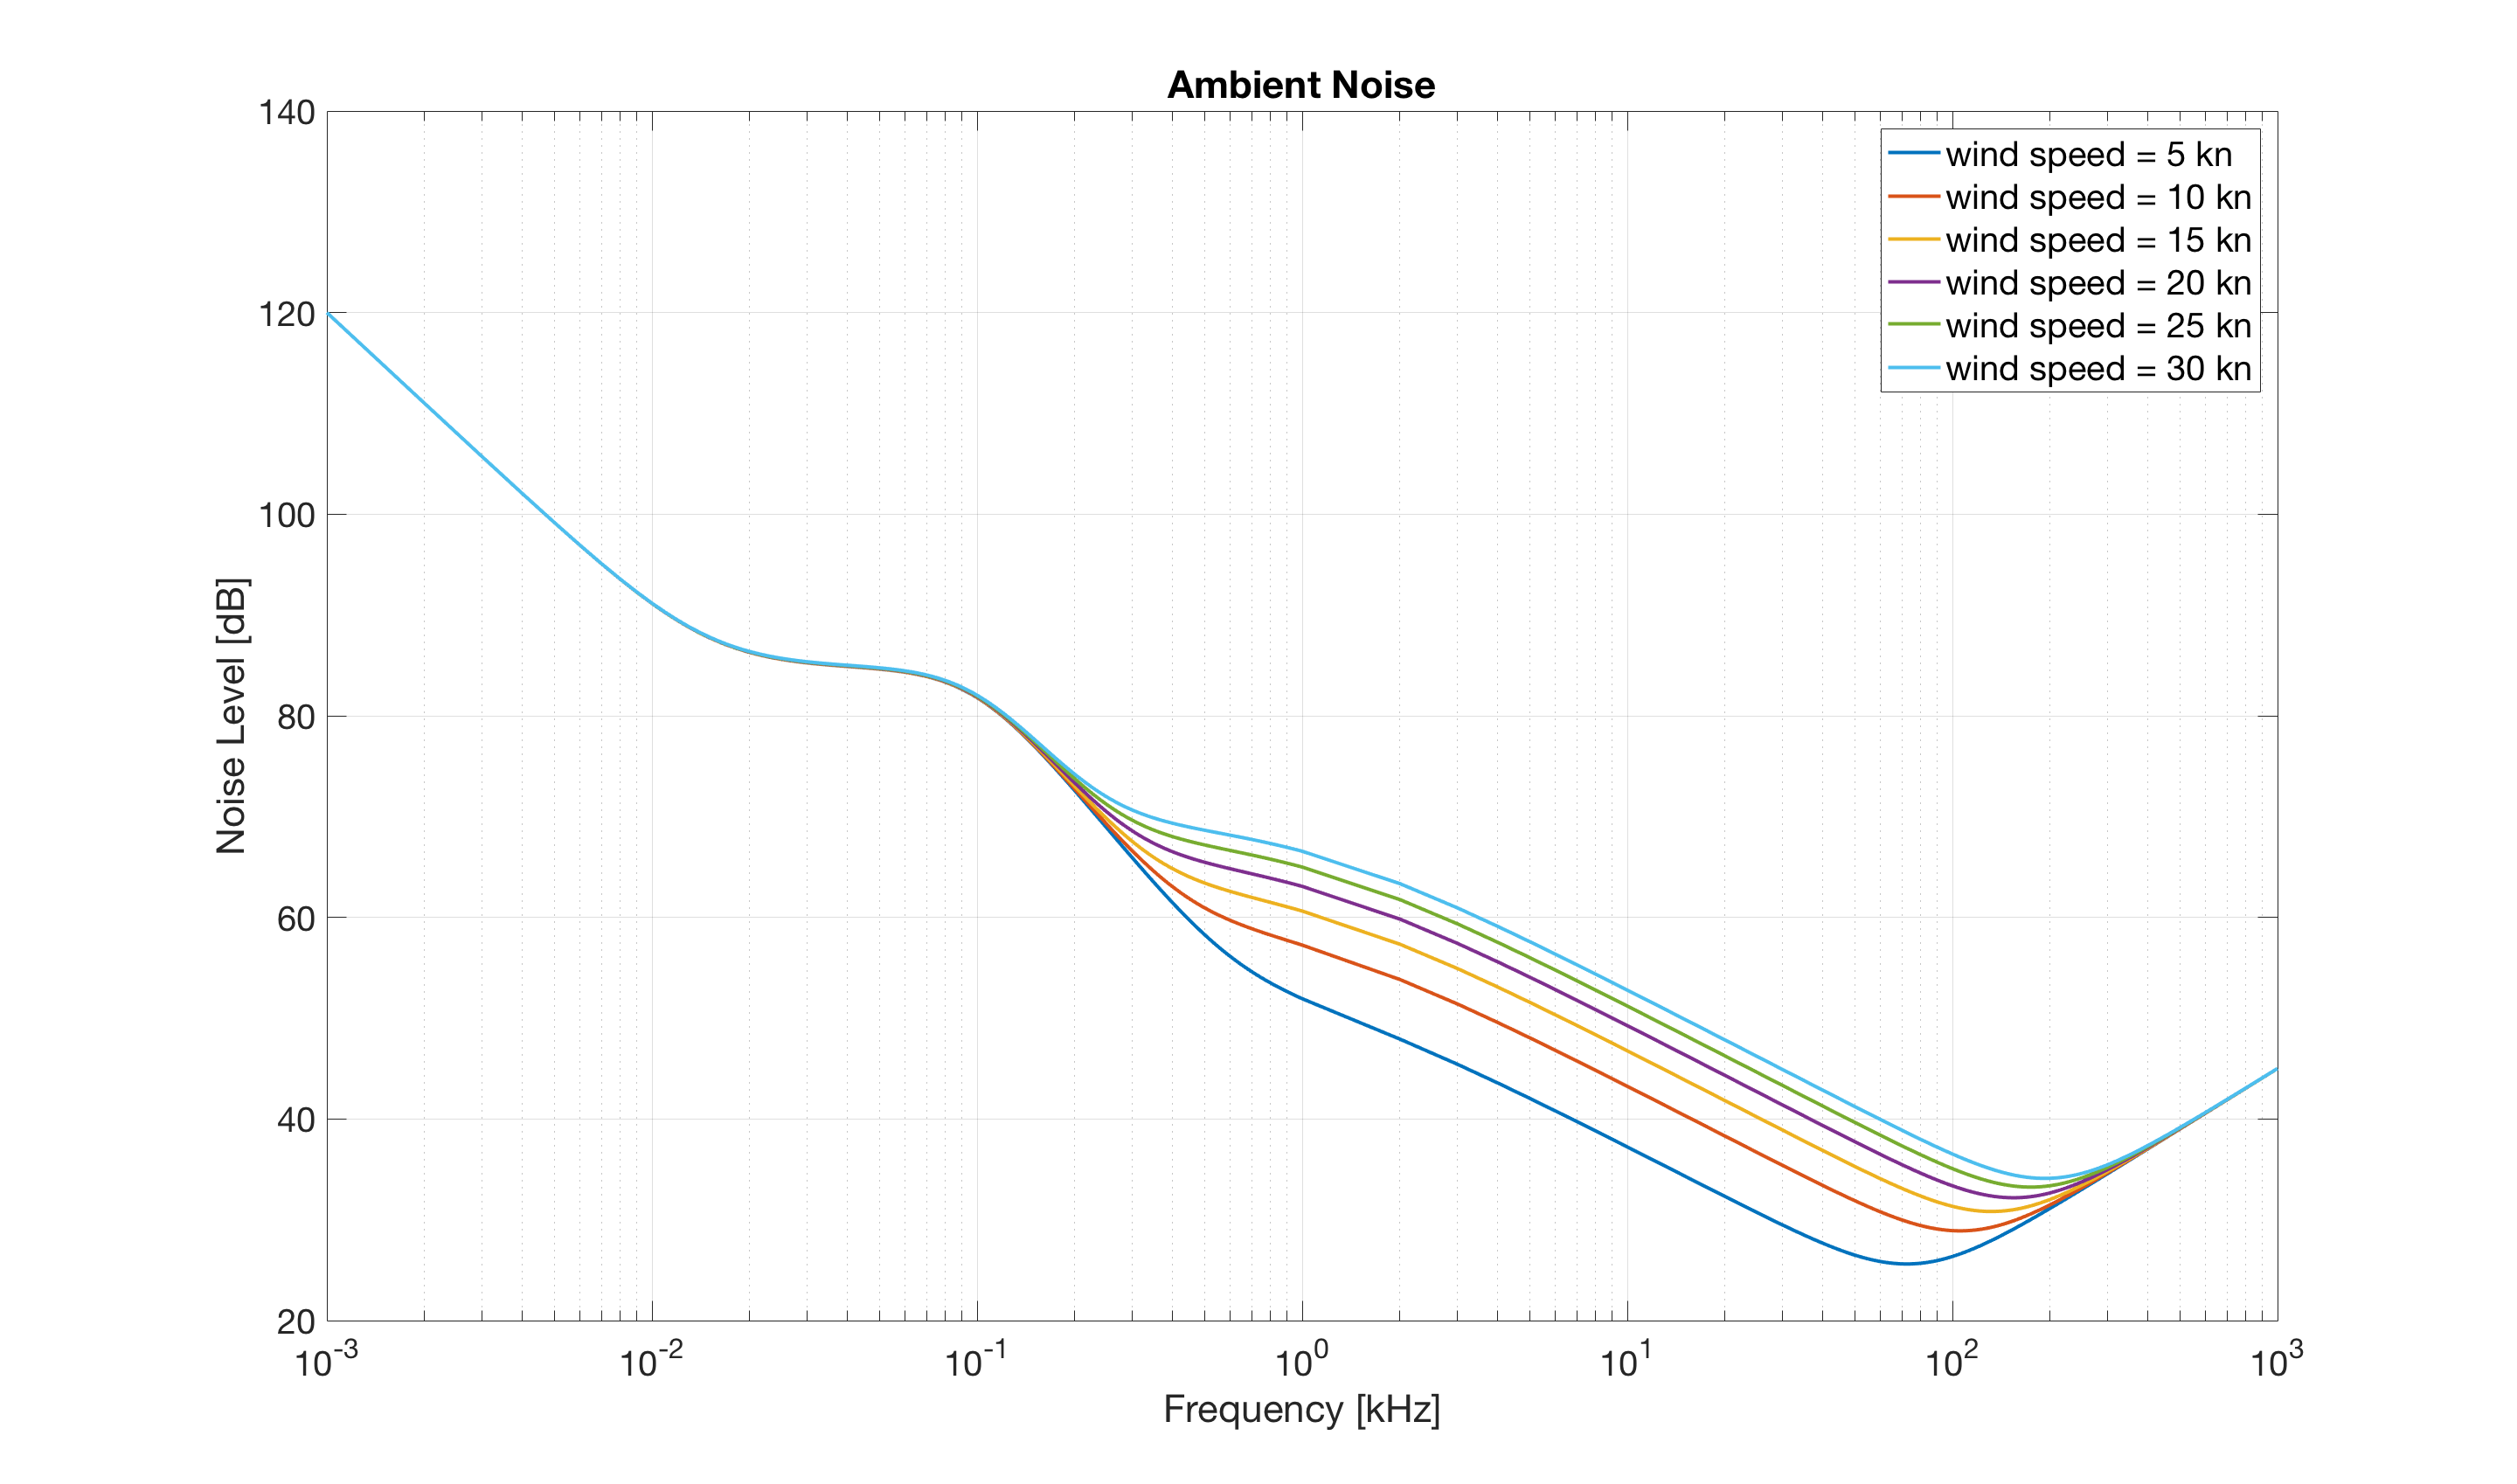
\includegraphics[scale=0.18]{usp4_1.png}}
\caption{Noise level dependency on wind speed and frequency}
\end{figure}

\section{ Contribution of different noise sources } \label{ Contribution of different noise sources } 
\noindent In-order to indicate the frequency domains where either traffic, turbulence, sea state or thermal noise level dominate, we assumed that contribution to noise from rainfall, shrimps and vessel are negligible. The noise isotropic levels for traffic, thermal, turbulence and sea state are computed by the mathematical models as explained in the theoretical section.  Also this was plotted for the wind speed of 5 kn.

\noindent  From the result shown in figure (2), we can distinguish different ambient noise, in different frequency range. We can observe the effect of turbulence noise between 1 Hz to 10 Hz. In the frequency range between 10 Hz to 300 Hz, the noise is affected by the traffic, shipping and harbours. Wind speed and sea state contribute the noise level from 300 Hz to 100 kHz. Above 100 kHz, noise level increases due to molecular agitation in the ocean. The random motion of water molecules causes thermal noise ultimately establishing the lower limit of measurability of pressure fluctuations associated with truly propagating sound waves above 100 kHz frequency. Isotropic noise level is shown by the superposition of all these effects in the graph. 

\begin{figure}[H]
\centering
{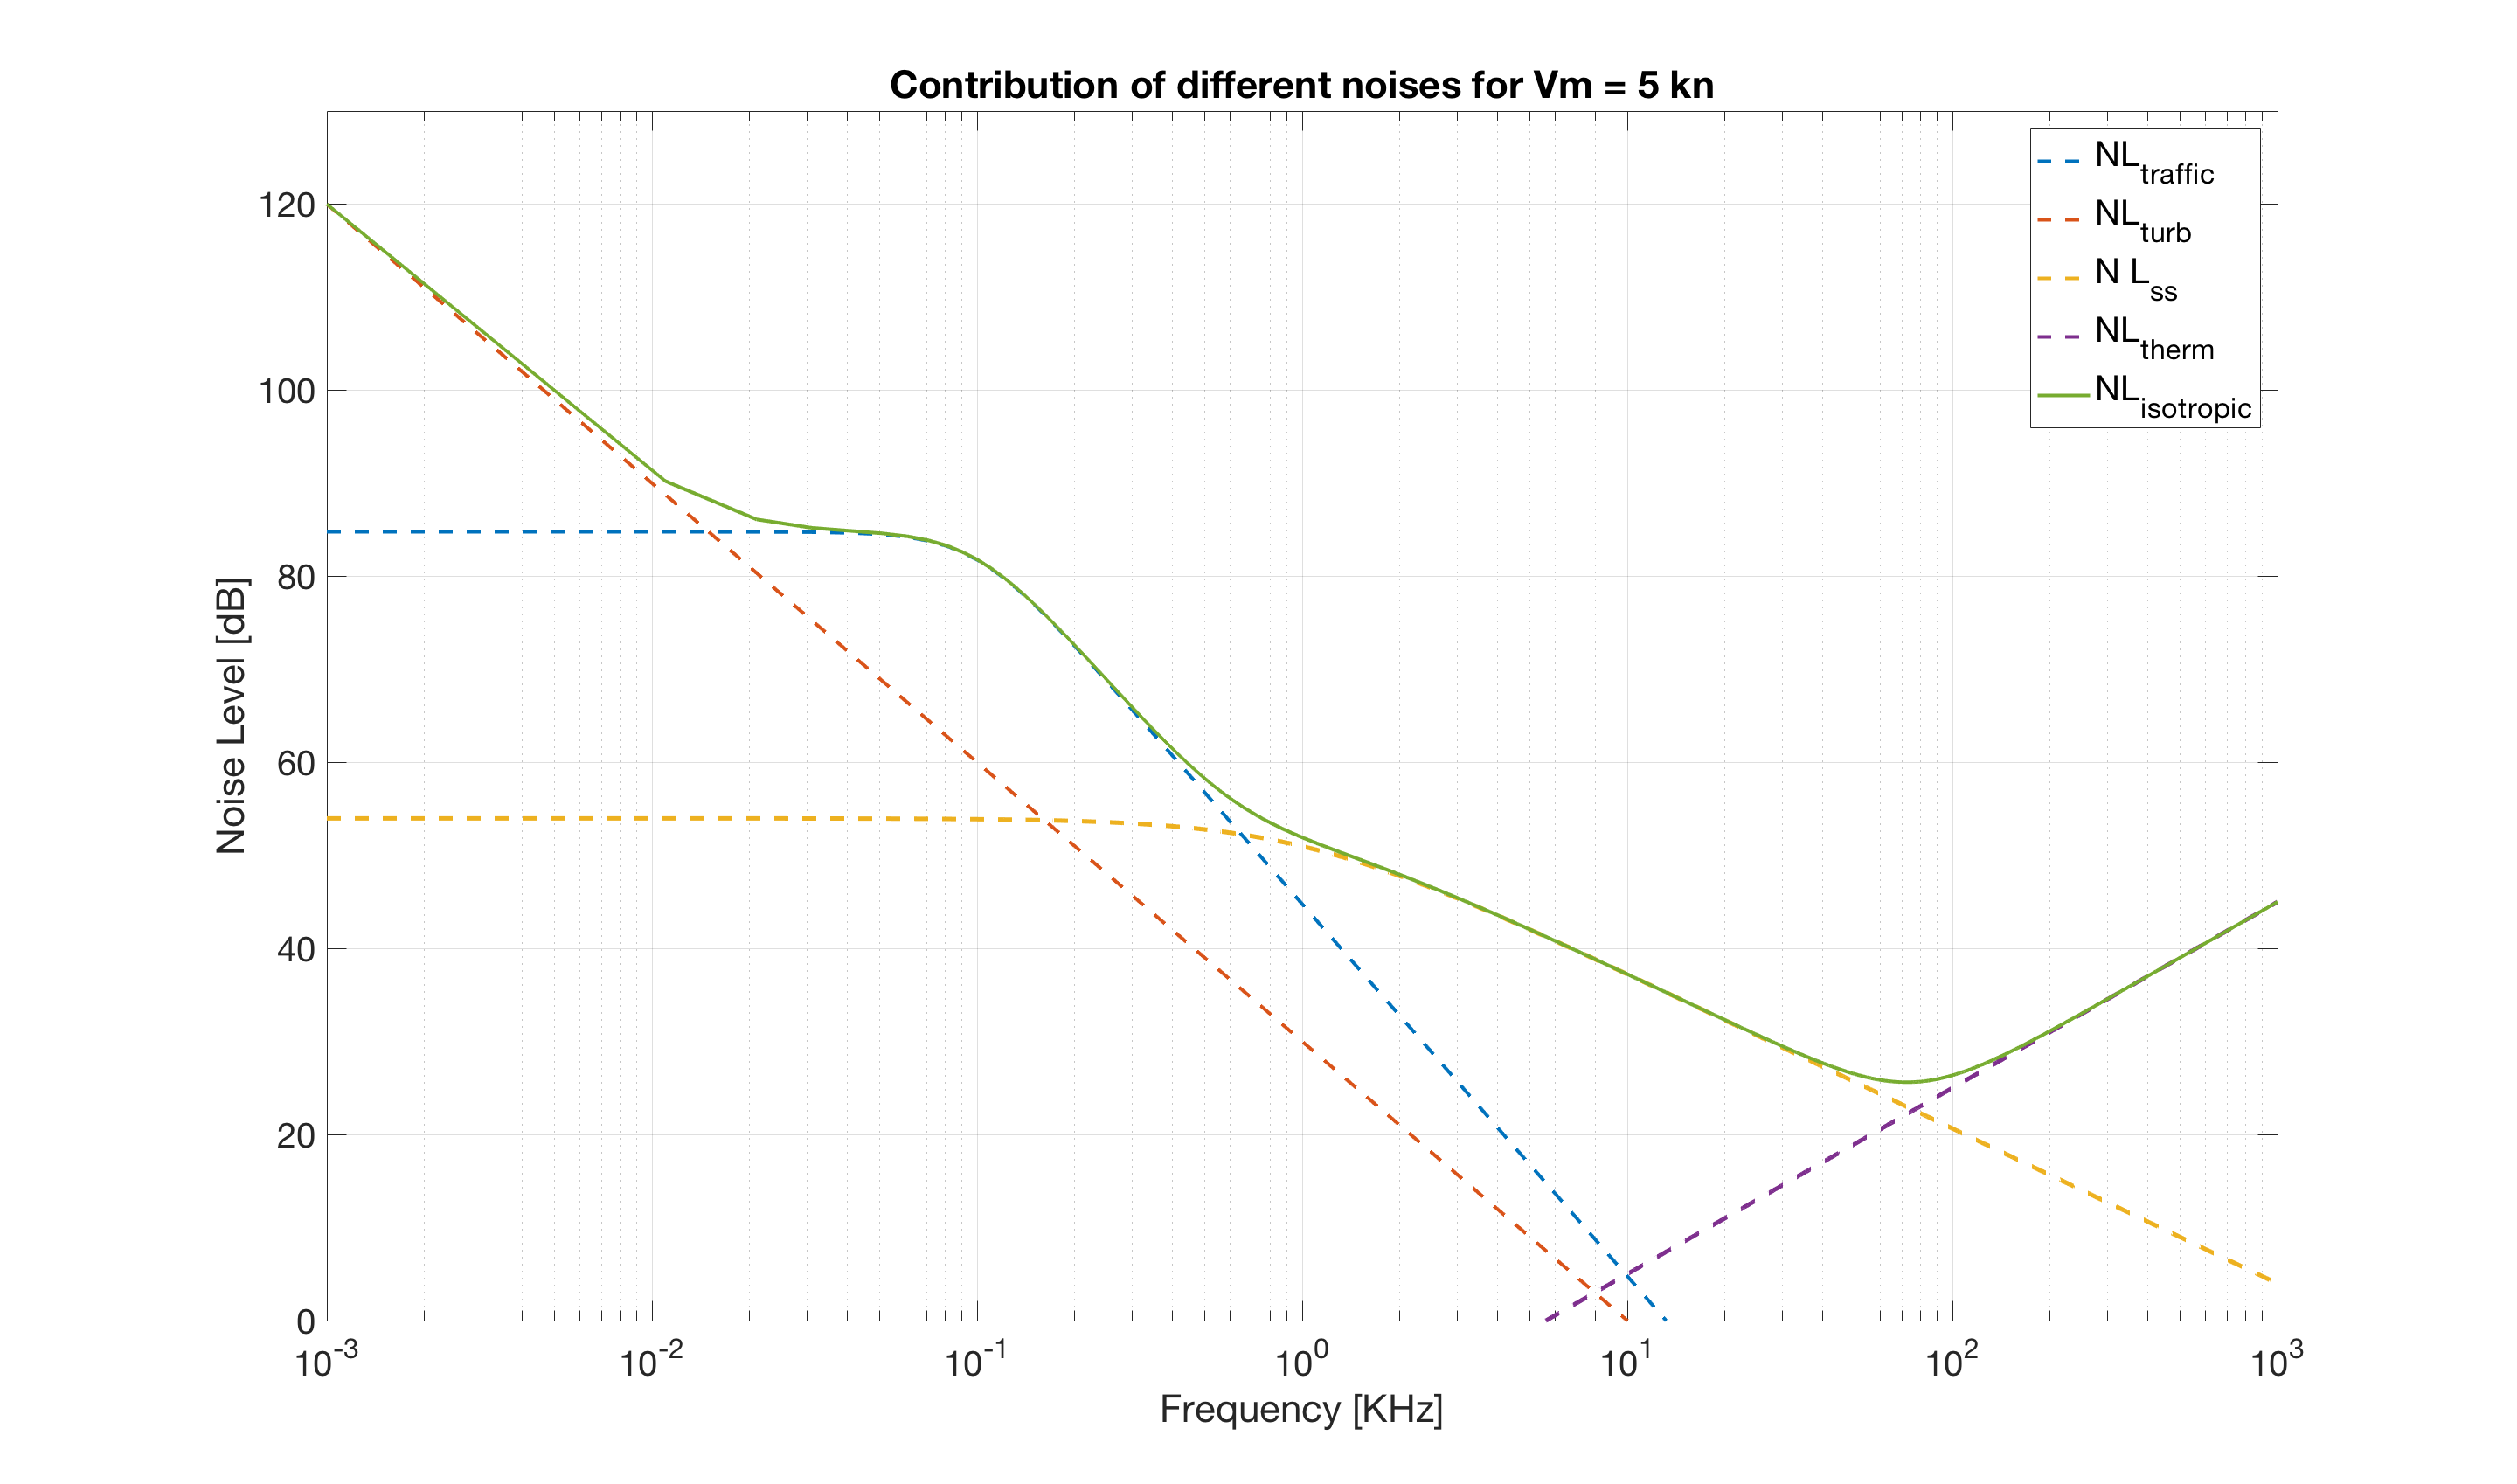
\includegraphics[scale=0.18]{usp4_2.png}}
\caption{ Contribution of different noise sources }
\end{figure}

